\section{Combinations}

    \subsection{What are Combinations?}
     A Combination is a way of selecting objects (permuting) from a group, without the order being important.
     In essence, it is orderless permutations. Let $ABC$ be a permutation.
     With permutations we asserted that $ABC$ and $BAC$ are different, as they are ordered differently.
     In combinations, we assert that $ABC$ and $BAC$ are the same, as they contain the same objects, just in a different order.

    \subsection{Set Theory}
    Set Theory involves the creation and manipulation of sets and their properties.
    A set is a collection of distinct objects in which their order does not matter.
    The objects in this set are called elements.
    If a set does not have any elements in it, we refer to it as a \emph{null set}, which is shown as $\emptyset$ or $(\emptyset)$.
    This null set is a subset of everything.
    If we want to describe a set containing elements, we must follow the example below.
    \begin{equation*}
        X = \{a,b,c,d,e,f,\cdots,y,z\}
    \end{equation*}
    If we wish to describe the number of elements in the set, we can use $n(X)$, where X represents the set, and n returns the number of elements in that set.
    In this case $n(X) = 26$, as set X contains all the letters of the alphabet.
    Sets are referred to differently when compared to other sets, as defined below.
    \begin{definition}
    Special Properties of Sets when Compared to Other Sets
    \begin{enumerate}
        \item If two sets have no elements in common they are called disjoint sets.
        \item If two sets have all elements in common they are equal.
        \item If all of elements of A are also in B then A is a subset of B $(A\subseteq B)$
    \end{enumerate}
    \end{definition}
    
        \subsubsection{Universal Set and Complement Sets}
        The set of all elements being considered is called the\emph{universal set} and is always denoted by $S$.
        When referring to a set of all elements that are in the universal set, but\textbf{ not in set A}, we call this the complement of $A$ or $A`$. For example:
        \begin{equation*}
            S = \{1,2,3,4\}, A = \{1,3\}, A`=\{2,4\}
        \end{equation*}
        
        \subsubsection{Unions and Intersections}
        For two sets of A and B, the \textbf{union} of A and B or $A\cup B$, is the set of all elements in A or B, not including duplicates.
        \begin{equation*}
            S = \{1,2,3,4\}, A = \{1,3\}, B =\{1,2\}, A\cup B=\{1,2,3\}
        \end{equation*}
        For two sets of A and B the \textbf{intersection} of A and B, $A\cap B$, is the set of all the elements that are in both set A and set B.
        \begin{equation*}
            S = \{1,2,3,4\}, A = \{1,3\}, B =\{1,2\}, A\cap B=\{1\}
        \end{equation*}
        If you are ever having trouble remembering the difference between the symbols representing the union and the intersection, remember that a union looks like a cup, and intersection looks like a cap.
        
        \subsubsection{Subsets}
        Subsets, are sets that are also in another set. To find every possible subset (including null set) we need to use the equation:
        \begin{equation*}
            2^{n(X)}
        \end{equation*}
        In this case, n(X) is the number of elements in Set X. If a question comes up, where we need the number of subsets of a given set with the length $y$, of set $x$, we'd simply use $\binom{n(x)}{y}$
        
    \subsection{Introduction to Combinations}
    A combination is a selection of r objects, from n distinct objects \emph{without regard for order}.
    The equation for solving combinations is written below.
    \begin{equation*}
        C(n,r) = \frac{n!}{(n-r)!\cdot r!}
    \end{equation*}
    This equations finds all combinations by dividing number of objects, by the unused objects $(n-r)!$ and the order of the selected objects.
    This can be further simplified to:
    \begin{equation*}
        C(n,r) = \frac{P(n,r)}{r!}
    \end{equation*}
    If order does not matter, the process is called a \emph{Combination}, whereas when order does matter, it is called a \emph{Permutation}.
    On your calculator, the formulae for combinations will be shown as \textbf{nCr}.
    If written out by hand, we will use the form:
    \begin{equation*}
        \binom{n}{r} = \frac{n!}{(n-r)!\cdot n!}
    \end{equation*}
    Or simply \(\binom{n}{r}\).
    
    \subsection{Inclusion\textemdash Exclusion Principle}
    The Inclusion-exclusion principle is a method of obtaining the number of elements in finite sets.
    Typically used when asked for the number of combinations of two things, where there is overlap between the two.\\
    Let A represent Set A, and let B represent Set B.
    \begin{center}
        %% Thank you http://tex.stackexchange.com/questions/9681/how-to-draw-venn-diagrams-especially-complements-in-latex
        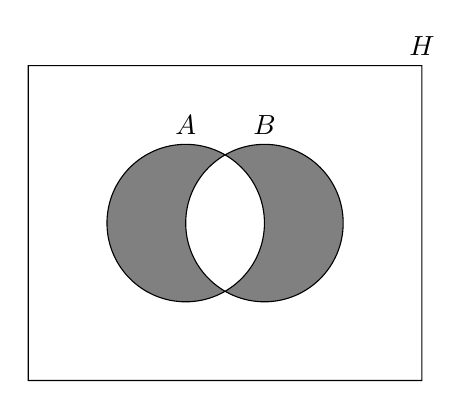
\begin{tikzpicture}[fill=gray]
            % left hand
            \scope
            \clip (-2,-2) rectangle (2,2)
                  (1,0) circle (1);
            \fill (0,0) circle (1);
            \endscope
            % right hand
            \scope
            \clip (-2,-2) rectangle (2,2)
                  (0,0) circle (1);
            \fill (1,0) circle (1);
            \endscope
            % outline
            \draw (0,0) circle (1) (0,1)  node [text=black,above] {$A$}
                  (1,0) circle (1) (1,1)  node [text=black,above] {$B$}
                  (-2,-2) rectangle (3,2) node [text=black,above] {$H$};
        \end{tikzpicture}
    \end{center}
    This diagram perfectly represents the overlap between the two sets.
    If you caught it earlier, what we're actually finding is $A\cup B$.
    The Inclusion\textemdash Exclusion Principle is merely a way of finding it algebraically.
    The image above represents the equation below.
    \begin{equation*}
        |A\cup B| = |A| + |B| - |A\cap B|
    \end{equation*}
    What happens if we have have three events we need to find the union of though?
    To do that, we'll follow the same principles, and use the equation below.
    \begin{equation*}
        |A\cup B\cup C| = |A| + |B| + |C| - |A\cap B| - |A\cap C| - |B\cap C| + |A\cap B\cap C|
    \end{equation*}
    %%TODO: Include a Venn Diagram for this equation above.